\documentclass[a4paper]{article}
\usepackage[left=1.0in, right=1.0in, top=1in, bottom=1in, includefoot, headheight=13.6pt]{geometry}
\usepackage{times}
\usepackage{tikz}
\usepackage[ruled,vlined,linesnumbered]{algorithm2e}
\usetikzlibrary{calc,arrows}
\parindent 0pt
\parskip 1.33ex
  
%% Begin
\title{BDI-Learning Discussion Paper \#6:\\A Robust \& Scalable Confidence Measure}

\author{
Dhirendra Singh\\dhirendra.singh@rmit.edu.au
}

\begin{document}

%\date{7 July 2009}

\maketitle


%%
\section{Calculating Plan Confidence}

Previously we have used the notion of coverage \cite{Singh:AAMAS10} and structural complexity \cite{Singh:HYCAS10} to capture the ongoing exploration of the goal-plan structure. The idea is that the extent of exploration of the structure in some way relates to how confident we are in the resulting decision tree. Both approaches depend on the calculation of the number of \textit{choices} below a plan in the goal-plan hierarchy. 

The main benefit of these coverage-based approaches is that they give a continuous confidence measure that is useful in fine-tuning exploration of the goal-plan structure. However the downside is that it is difficult to calculate (1) the full set of paths (specially when parameterised and recursive goals are considered); and (2) which path combinations beginning in a failed trace should be ``counted'' as covered since some combinations never eventuate.

Compare this to \textit{stability} \cite{Airiau:IJAT09,Singh:AAMAS10}, a boolean measure of confidence that is not very useful for guiding exploration, nonetheless is effectively equivalent to coverage \cite{Singh:AAMAS10} only without the complication of paths calculations.

In this section, we explore a confidence measure that combines the merits of both the coverage-based and stability-based measures. The idea is that confidence for a plan $P$ in a given world $w$ may be defined as \textit{the ratio of the number of stable plans below $P$ to the total number of plans tried below $P$, starting in world $w$}. In other words, our confidence gradually increases as plans below $P$ start to become stable, and is maximum when every plan that has been tried below $P$ is considered stable.


\begin{figure}[ht]
\begin{center}
\resizebox{.75\textwidth}{!}{%!TEX root = ./dp6-confidence.tex

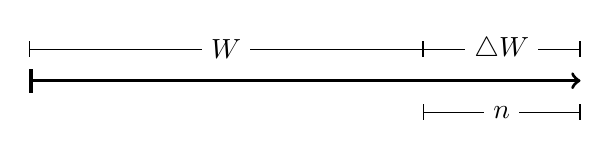
\begin{tikzpicture}
\draw[|->,very thick] (0,0) -- (7,0);
\draw[|-|,>=angle 90] (5,-0.4) -- (7,-0.4) node[midway,fill=white]{$n$}; 
\draw[|-|,>=angle 90] (0,0.4) -- (5,0.4) node[midway,fill=white]{$W$}; 
\draw[|-|,>=angle 90] (5,0.4) -- (7,0.4) node[midway,fill=white]{$\triangle W$}; 

\end{tikzpicture}


}
\end{center}
\caption{An example goal-plan hierarchy.}
\label{fig:conf}
\end{figure}

Let us consider the example goal-plan structure of Figure \ref{fig:conf}, and see how the confidence calculation might work for the top-level plan $P$. Let's say the first execution results in the failed trace $\lambda=G[P:w] \cdot G1[P_1:w] \cdot G3[P_7:w]$. The confidence in $P$ is then:

\begin{equation}
confidence(P,w)=\frac{stable~plans~in~[P,P_1,P_7]}{total~plans~in~[P,P_1,P_7]} = \frac{0}{3}
\end{equation}

Let's say the second execution results in the failed trace $\lambda=G[P:w] \cdot G1[P_2:w]$. The confidence at this step is then:

\begin{equation}
confidence(P,w)=\frac{stable~plans~in~[P,P_1,P_2,P_7]}{total~plans~in~[P,P_1,P_2,P_7]} = \frac{0}{4}
\end{equation}

Now, let's say the next four executions fail in $P_2$, $P_8$, $P_2$ (that becomes stable), $P_4$ (note that for this to happen $P_9$ must have been selected first). At step six then, the confidence is given by:

\begin{equation}
confidence(P,w)=\frac{stable~plans~in~[P,P_1,P_2,P_4,P_7,P_8,P_9]}{total~plans~in~[P,P_1,P_2,P_4,P_7,P_8,P_9]} = \frac{1}{7}
\label{eqn:conf3}
\end{equation}

And so on. 

In Figure \ref{fig:conf}, the number against each plan node $P*$ indicates the maximum number of sub-plans that will eventually be considered at that node for full confidence. Algorithm \ref{alg:conf} describes this confidence calculation for a given active execution trace $\lambda$. Here $\eta$ is used to propagate the full list of sub-plans in the trace up to the parent. $StablePlan$ is a boolean function to check if the given plan $P_n$ is stable r not. $Choices$ holds the full list of all past sub-plans executed along with their stability status.

\begin{algorithm}[ht]
\KwData{$\lambda=G_0[P_0:w_0] \cdot \ldots \cdot G_n[P_n:w_n]$; $\eta=[P,b] \cdot \ldots \cdot [P_{r},b_{r}]$; $k\geq0$; $\epsilon\geq0$}
\KwResult{Updates confidence for plans in $\lambda$}
$choices(P_n,w_n) = choices(P_n,w_n) \cup P_n \cup \eta$\;
$confidence(P_n,w_n) +\!\!= |choices(P_n,w_n) == true|/|choices(P_n,w_n)|$\;
\If{$|\lambda| > 1$}{
	$\lambda'=G_0[P_0:w_0] \cdot \ldots \cdot G_{n-1}[P_{n-1}:w_{n-1}]$\;
	$\eta'+\!\!=[P_n,StablePlan(P_n,k,\epsilon)]$\;
	$UpdateConfidence(\lambda', \eta', k, \epsilon)$\;
}
\caption{$UpdateConfidence(\lambda, \eta, k, \epsilon)$}
\label{alg:conf}
\end{algorithm}

The first benefit of this approach is that the confidence grows gradually, in a manner similar to coverage, and may be used to similarly guide exploration. The second benefit is that we do not have to concern ourselves with possibilities (paths) that may never eventuate, as we do with coverage. Say if plan $P_9$ was to also fail in world $w$. In that case goal $G_2$ would never be posted and all it's sub-plans would never be executed. For coverage-based calculations this is a problem since we consider the full gamut of possibilities, and ignoring such combinations would mean that full coverage would never be achieved. With this new measure however, since we only deal with past occurrences then we are still guaranteed to converge to full confidence as long as the set of previously tried plans are executed sufficient times to become stable. The third benefit is that the method scales well as it does not depend on the complexity of the domain, but only on the execution history.

One limitation of this (and our previous approaches) is that the confidence measure is a per-world concept while the decision tree that it is applied to encapsulates knowledge from multiple worlds. This means that if a new world is witnessed, then even though the decision tree might generalise based on past worlds, the confidence measure will always be zero resulting is the plan selection weight to default to $0.5$. One way to improve this situation for unseen worlds would be to use an average confidence value from all previously seen worlds. This would allow generalisations to be used, but with some reservation based on confidence.

\fbox{To Resolve: $P_9$ is not part of the active execution trace ending in $P_4$ so will be missed in Equation \ref{eqn:conf3}.}

\section{Calculating Domain Confidence}

Here, instead of determining our confidence in the plan (based on exploration of the structure), the aim is to build a confidence measure to capture the complexity of the domain (i.e number of worlds). The motivating idea for the solution is that a confidence measure may be constructed around the rate at which new worlds are being witnessed by a plan. During early exploration it is expected that the majority of worlds that a plan is selected for will be unique, therefore this rate is high and our confidence is low. Over time as exploration continues, the plan would get selected in all possible worlds and the rate of new worlds would taper off towards zero. Intuitively, our confidence over this period would increase to it's maximum. 

\begin{figure}[ht]
\begin{center}
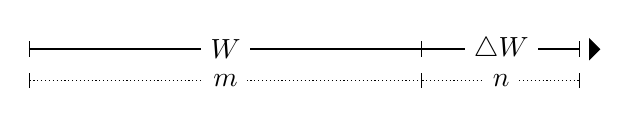
\begin{tikzpicture}
\draw[-, thick] (0,0) -- (7,0);
\draw[->,>=triangle 90] (7.25,0) -- (7.26,0);
\draw[densely dotted,|-|,>=angle 90] (0,-0.4) -- (5,-0.4) node[midway,fill=white]{$m$}; 
\draw[densely dotted,-|,>=angle 90] (5,-0.4) -- (7,-0.4) node[midway,fill=white]{$n$}; 
\draw[|-|,>=angle 90] (0,0.0) -- (5,0.0) node[midway,fill=white]{$W$}; 
\draw[-|,>=angle 90] (5,0.0) -- (7,0.0) node[midway,fill=white]{$\triangle W$}; 
\end{tikzpicture}
\end{center}
\caption{Passage of worlds with time for a given plan.}
\label{fig:domain_confidence}
\end{figure}

In inverse terms, confidence would increase with the rate at which old worlds are being witnessed. Figure \ref{fig:domain_confidence} illustrates the passage of time from the point of view of a given plan. Here $W$ is the set of all worlds witnessed in the first $m$ experiences and $\triangle W$ is the set of worlds witnessed in the last $n$ experiences. Then $|W \cap \triangle W|$ gives us the number of old worlds seen in the last $n$ experiences. For a given plan $T$, Equation \ref{eqn:domain_confidence} gives the ratio that defines our domain confidence measure $0 \leq \kappa_T \leq 1.0$ that is guaranteed to converge to $1.0$ if $n<=m$ and as long as all worlds are eventually witnessed. The value $n$ may be computed as $n=a \cdot m$ where $0.0 < a \leq 1.0$ is a user-specified option.


\begin{equation}
\kappa_T = \frac{| W \cap \triangle W |}{n}
\label{eqn:domain_confidence}
\end{equation}


\section{Putting It all Together: Calculating Plan Selection Weight}

For plan $T$, the plan confidence $c_T(w)$ and domain confidence $\kappa_T$ may then be used to calculate a final plan selection weight $\Omega(w)$ as given by Equation \ref{eqn:omega}. Here $p_T(w)$ is the probability of success in world $w$ given by the decision tree of plan $T$.


\begin{equation}
\Omega'_T(w) = 0.5 + \left[  c_T(w) *  \kappa_T * \left( p_T(w) - 0.5 \right)  \right].
\label{eqn:omega}
\end{equation}


%%
\begin{thebibliography}{10}

\bibitem{Airiau:IJAT09}
S.~Airiau, L.~Padgham, S.~Sardina, and S.~Sen.
\newblock Enhancing Adaptation in {BDI} Agents Using Learning Techniques.
\newblock In {\em International Journal of Agent Technologies and Systems},
2009.

\bibitem{Singh:AAMAS10}
D.~Singh, S.~Sardina, L.~Padgham, S.~Airiau.
\newblock Learning Context Conditions for {BDI} Plan Selection.
\newblock In {\em Proceedings of Autonomous Agents and Multi-Agent Systems (AAMAS)}, 2010.

\bibitem{Singh:HYCAS10}
D.~Singh, S.~Sardina, L.~Padgham.
\newblock Extending BDI Plan Selection to Incorporate Learning from Experience.
\newblock Submission under review for the Special Issue on Hybrid Control of Autonomous Systems (HYCAS), Journal of Robotics and Autonomous Systems, 2010.


\end{thebibliography}

\end{document}